\chapter{Engine architecture overview}

Now, after the last chapter described many different kinds and sizes of engines, this section is going to examine the architecture that powers an engine. At the beginning an overview of a modern game engine's runtime architecture is given. That overview is then followed by a description of several selected submodules. These power different systems of the engine and are responsible for its performance and functionality. The submodules were chosen based on the author's opinion of their relevance and importance to the backbone of an engine.

\section{General runtime architecture} \label{engine_runtime_arch}

When talking about software parts of an engine in a high level fashion it can be separated into two clearly diverging parts, tools and the runtime component. This section will almost entirely discuss the runtime part while only mentioning the most important tools at the end. An engine consists from many modules which are separated into different layers. Game engines share this architectural design decision with many other software projects that reach a specific size. Layers group modules together with other ones operating in the same order of magnitude as their siblings. A layer often depends upon lower ones but shall not have any dependencies to upper ones. This ensures that coupling between layers is loose which leads to more stable software solutions. An exemplary illustration of a generic engine's runtime architecture can be seen in Figure \ref{fig:engine_runtime_arch}.

\begin{figure}[h!]
	\centering 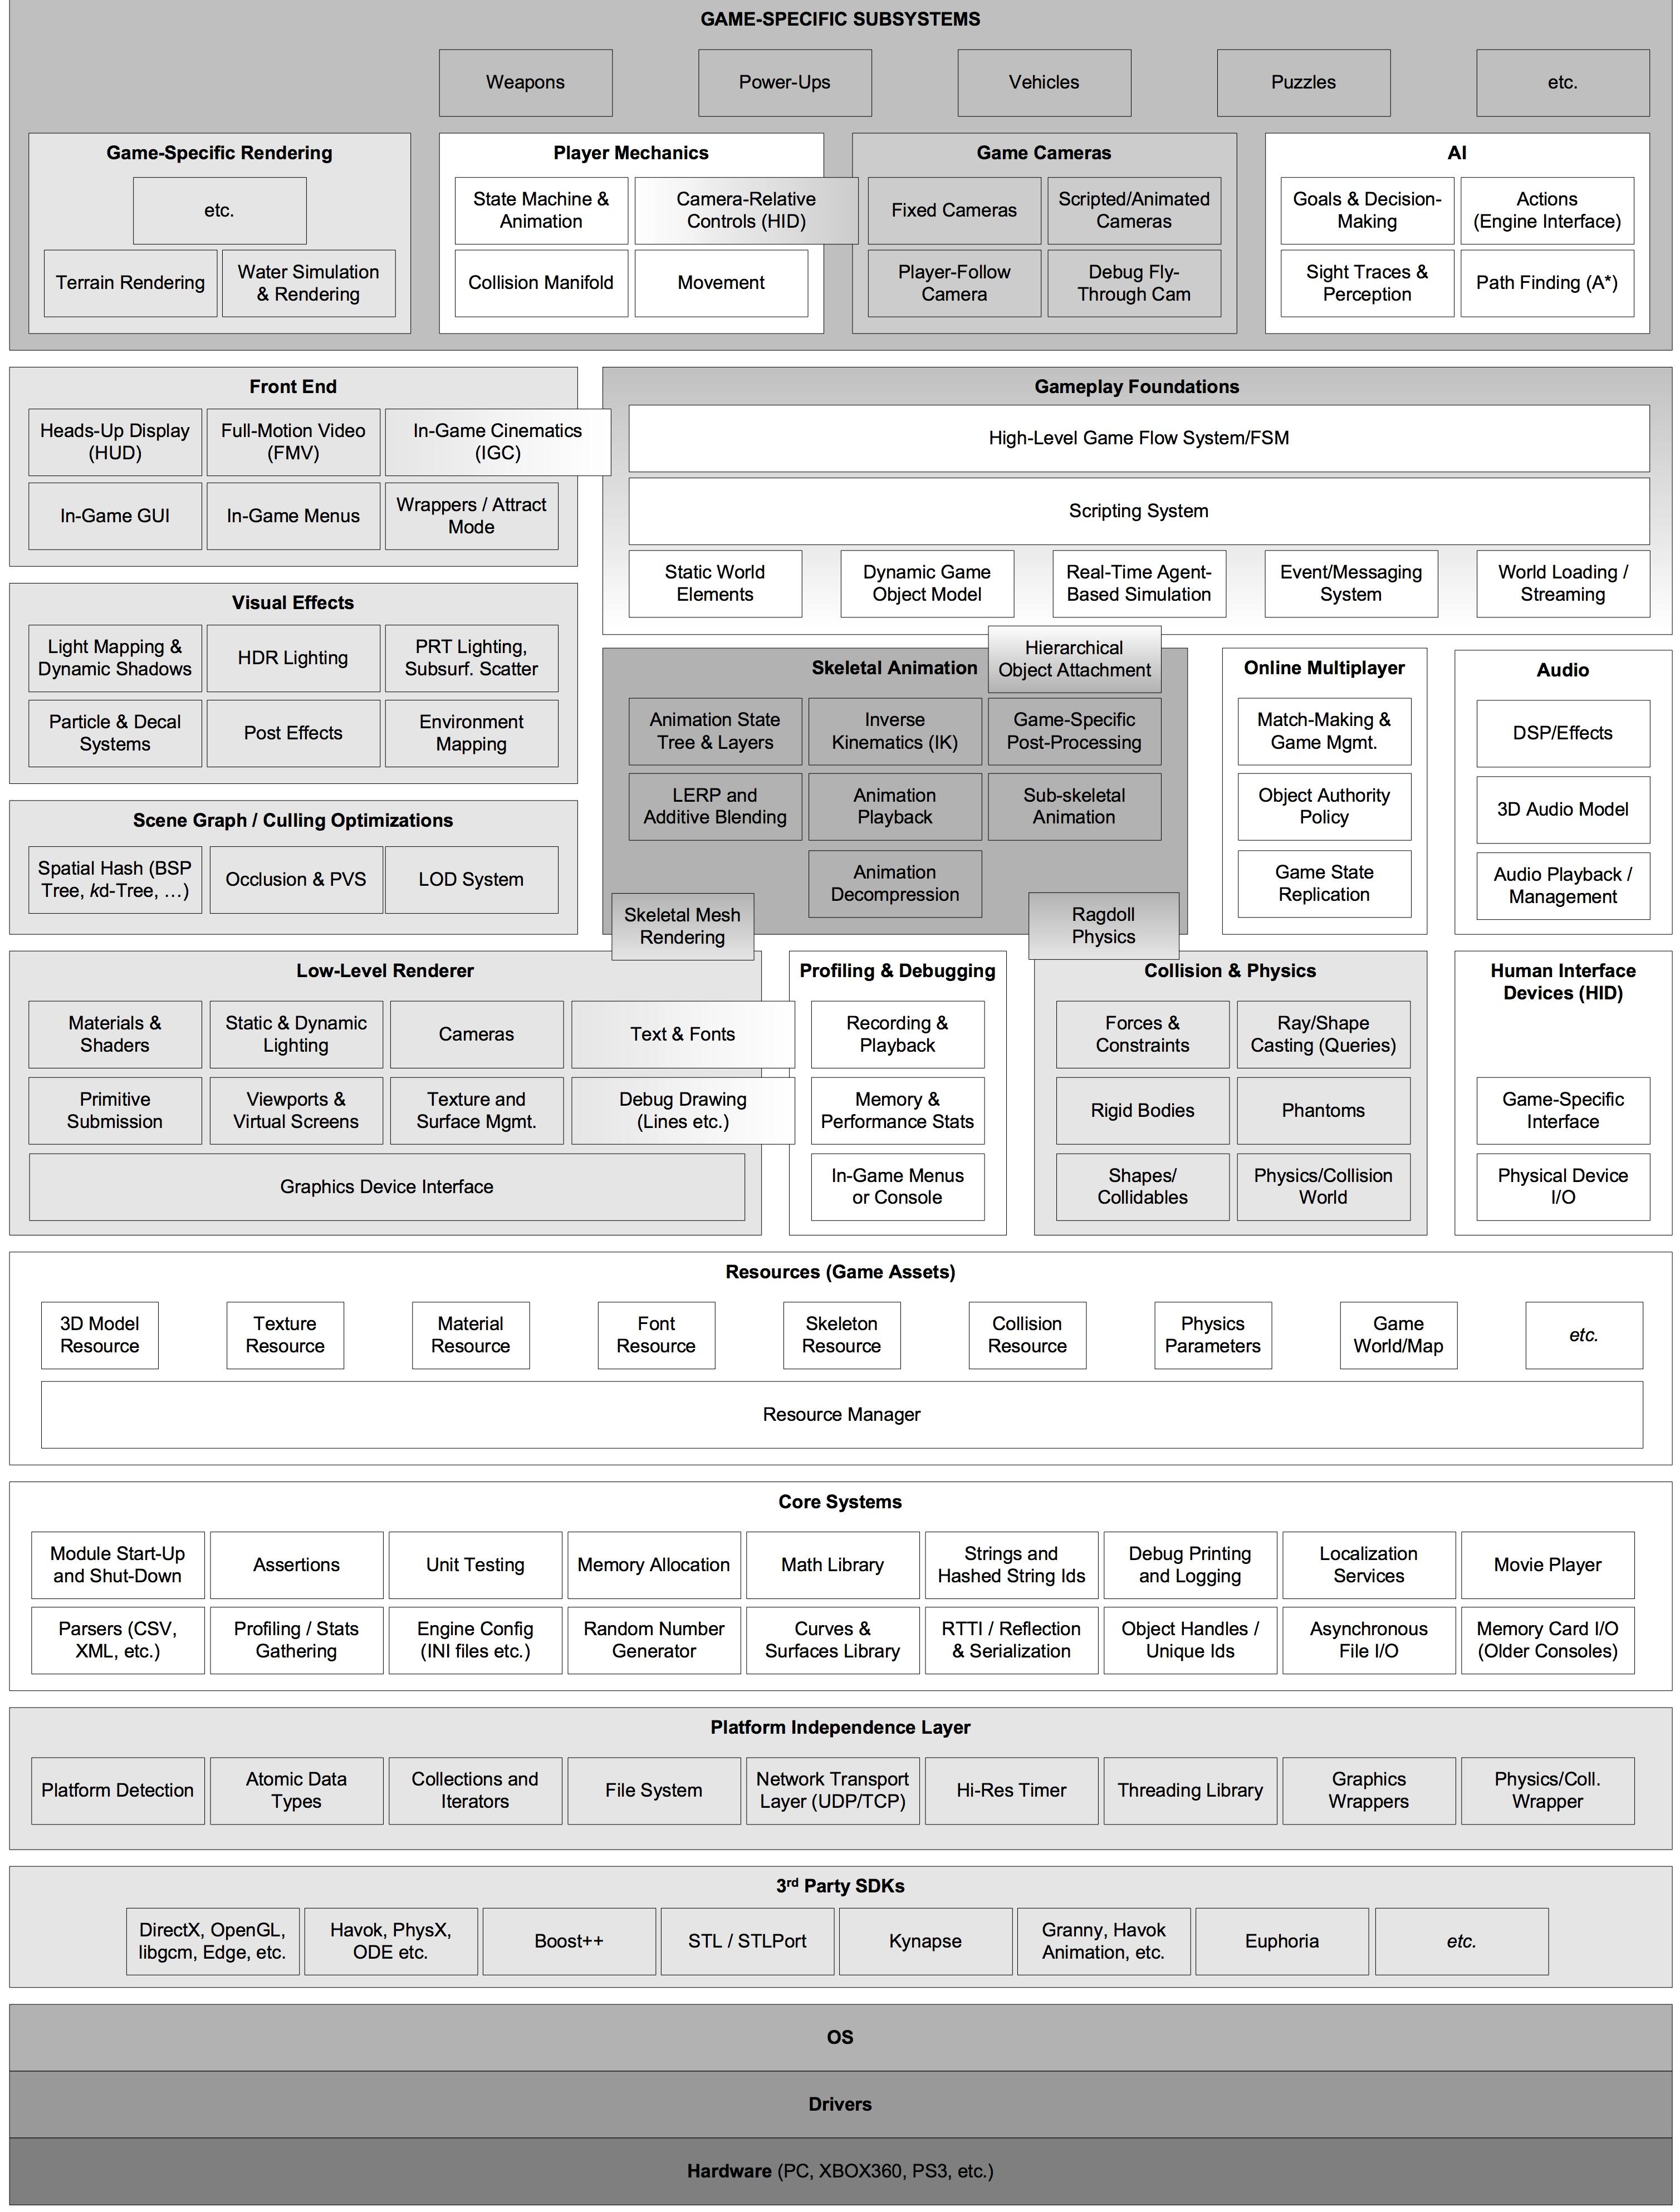
\includegraphics[width=\linewidth]{PICs/engine_runtime_arch.jpg}
	\caption{Illustration showing common modules grouped into distinct layers of a large scale engine solution}
	\label{fig:engine_runtime_arch}
\end{figure}

The complexity of modules in a layer grows when ascending through them from bottom to top. Where the lowermost layers include low-level systems essentially drivers \footnote{A program that controls or communicates with a hardware device}, platform-dependent 3\textsuperscript{rd} party \acp{SDK} or platform-independent abstraction components. Traversing the hierarchy upwards from core systems, over resource management, to general rendering and gameplay foundation modules, at one point the uppermost layers are reached. Those encompass game specific subsystems that can vary from one game to another. With the crude knowledge of the different layers involved in an engine it can be emphasized that a game engine is a highly complex software and building one is an endeavor that requires expertise, experience and time. It is important to properly reason out the architecture and uphold the focus onto the engine's goal. Maintaining focus while following the sketched out architecture will help to avoid unnecessary coupling and the implementation of irrelevant features or systems. 
The rest of this section will describe some modules from Figure \ref{fig:engine_runtime_arch} in-depth to investigate how they work and how they contribute to the combined whole.

\section{Memory Management}

One key constraint nearly every engine ha+s to fulfill is running games with a high frame rate. Because games are real-time simulations the time window for running gameplay logic and rendering a single frame is very limited. To complement this with discrete numbers for a game, running with 60 \ac{FPS} a slice of 16.6 ms can be used per single frame. To stay into this limits game developers came up with optimization techniques and algorithms that speed up calculations and processing. But the performance of code is not only dependent upon the efficiency of an applied algorithm but also how the program manages and uses its resources, especially memory. Controlling how an engine utilizes the \ac{RAM} is mandatory for guaranteeing high performance. The two most commonly applied memory usage optimizations are either reducing the amount of dynamic allocations at a game's runtime or allocating bigger sections of memory to store data in contiguous blocks. To solve these problems engines often implement custom memory allocators that have a better runtime performance then using the existing system allocator.

\subsection{Custom allocators}

Custom allocators are facilities that optimize dynamic memory allocations and reduce the performance penalty introduced by them. Its an allocator's main purpose to provide a source of memory the requester can work with. The process of finding a block of memory that fits the request is called an allocation. When requested memory is not needed anymore, the allocator takes it back and reuses it for another request if possible.
Almost all system programming languages come with a heap allocator, that can handle requests for memory at runtime. These so called \textit{heap allocations} are made by either calling \texttt{malloc() \& free()} (C) or \texttt{new \& delete operators} (C++). But caused by different aspects these allocations are rather slow. The performance penalty is mainly caused by two factors. At first, because any size of allocation has to be fulfilled by a heap allocator, it needs a lot of internal allocation management which introduces an overhead, making heap allocations costly. The second factor that contributes to the cost of dynamic allocations is that a context switch from user-mode to kernel-mode takes place before any allocation. 

To better understand why this introduces a performance penalty one has to know what divides the user- and kernel-mode. Many modern \acp{OS} distinguish between these two modes. A process, that is running in user-mode, often has no capabilities to directly talk with the underlying hardware, both for security and portability reasons. The way a user-mode process communicates with lower level systems is by issuing a \textit{system call}. Such calls trigger routines in the hardware that switches into the privileged kernel-mode, executing the requested kernel procedure while strictly controlling what is happening. After it terminates, the procedure forces a switch back into user-mode and the process continues at the point right after the system call.\cite{LinuxKernel}

And it is that context switching on system calls that slows down dynamic memory allocations. Whenever a call to \texttt{malloc()} or similar is issued, under the hood it forwards the request to a system call and the allocation is fulfilled in kernel-mode. But because every game engine needs some kind of dynamic allocations in some places, they have to be optimized. The common solution for this problem is a collection of customer allocators implemented in the engine's core systems. They resolve the problems bound to dynamic allocations by minimizing context switches and knowing the allocation patterns.
To reduce the overhead of system calls custom allocators satisfy allocation requests from a preallocated block of memory. This block can be acquired by the system's heap allocator (or with another approach that is described in the implementation section in chapter 6). After that block was allocated every further request for memory will stay in user-mode. Assuming the usage patterns of itself, a custom allocator can handle requests more efficiently than the general purpose heal allocator. Several different kinds of allocators are implemented and the user is responsible for knowing how the memory is used and which allocator fits the job best. That allows for reducing book keeping overhead and for better performing allocations.

The memory management module of a modern engine has a huge impact onto the general performance. It serves as the basis for many other modules and more high level ones, such as for example a container library, can be built on top of it. Being one of the modules that were implemented in the thesis' project, an even more in-depth insight into the internals of such a system and how it is implemented in Rust and C++ will be given in section \ref{mem_impl}. It will also describe how the different kinds of allocators work internally and how they can be easily combined with other utilities to form a versatile and well-performing system.

\section{Rendering}

One of the most complex parts of a game engine is the renderer. It encompasses many disciplines from graphics programming to algorithmic knowledge and there are many different architectures to choose from. This section will give a basic overview of how a renderer can be built but going into detail would quickly exceed the intention of this section. 
As many software solutions that become complex over time, a renderer is often separated into different layers. To recap them in a visually form, one can find them in Figure \ref{fig:engine_runtime_arch} under section \ref{engine_runtime_arch}. At the bottom of the architecture there is the low-level renderer. Its purpose is to render geometric primitives \footnote{Common primitives are points, lines or triangles} as quickly as possible without performing any redundant passes. To display the primitives onto a screen a renderer uses Graphics-\acp{SDK} such as OpenGL or DirectX. Cross-platform engines abstract the graphics \ac{API} used on a specific platform behind a layer called the \textit{graphics device interface}. This name is not a standard and can be any other one in the source code of different engines. It is the task of this interface to enumerate the available graphics devices and setup surfaces \footnote{Buffers on the \ac{GPU} into which the renderer stores its generated values}. Other components of the low-level renderer are for example a system to calculate dynamic and static lighting of the scene or a material system for managing shaders and hardware state on a per primitive basis. Shading and lighting are broad topics and an in-depth description is omitted on purpose due to the complexity of these fields. 
On top of the low-level renderer another layer is often implemented to decide, which primitives to process and submit. This higher level layer manages what primitives should be rendered based on visibility determinations. Some components that are included in this layer are a \ac{LOD} system. This systems is an optimization often used to reduce the amount of primitives for a mesh based on its distance to the camera. A model is replaced by a lesser detailed one the further away the camera is moving. If the distance is reduced again, the model is switched back to the more detailed version. Other exemplary techniques are \textit{frustum culling}, where objects that are not 'seen' by the camera are removed, or some kind of \textit{spatial subdivision}, where the virtual world is divided into smaller chunks which makes it more easy to reason about parts of the world that cannot be seen from a specific camera location.
Additionally to the described components a rendering engine can include systems to handle various special effects and post processing effects, such as dynamic shadows, particle systems and more realistic lighting techniques. It is often also capable of rendering some kind of \ac{UI} on top of the game's 3D scene. 

\section{Gameplay systems}

Beside the low-level systems an engine has to provide a possibility for game developers to define the rules and attributes of the game world and what abilities a player has. This action and logic, often called gameplay, is implemented in the engine's native or a more higher level scripting language. To allow gameplay code to interact with lower level systems from the engine's core, a layer called \textit{gameplay foundations} is introduced. What exactly is grouped into that layer differs from engine to another but two components that are found in any engine are some kind of scripting environment and a system for handling game objects and components.

\subsection{Game objects \& components}

Every game engine has some facility for representing an object in the virtual world. These so called \textit{game objects} can be crated and configured by game designers using the world editor or similar tools. But the implementation details on how these objects are modeled in code is quite complex and several different architecture techniques exist. 

\subsubsection{The object-centric approach}

The first and most straight forward approach is the object-centric one. With this technique every object in the game world is an instance of a class. This class contains both, attributes and logic of the object and one instance is created for every logical game object that is added to the world. That idea of grouping data and logic together into a single package is inherently similar to the way object oriented languages work. It is due to this similarity that leads game developers to often implement a hierarchy of game objects using inheritance. Such class hierarchies usually define a root class called \texttt{GameObject} that serves as a parent for every object in the world. The exemplary sub classes \texttt{PhysicsObject} and \texttt{RenderableObject} both are implemented as child classes to \texttt{GameObject}, having common functionality already defined in the parent class. While such a system can be intuitive and simple for a small hierarchy, as soon as complexity increases, the hierarchy starts getting deeper and its advantages fade away. With growing complexity the disadvantages of a class based solution become visible. A deep hierarchy of classes is inflexible to change requests. If a feature is requested, that does not fit into the already existing taxonomic system, it requires a lot of work or a non optimal workaround, to force the new requirement into the current model. 
A different problem that often arises with such a design is called the \textit{Bubble-Up effect}. When the number of different classes grows it is more likely that similar routines are implemented in several classes. In order to reuse existing code and to provide the designers with a possibility of applying the logic to other objects of the hierarchy, some routines and data are moved into the parent class. This is a problem because in the moment when the functionality is moved into the base class it is automatically available to all children of it, even to those who were never meant to gain that certain behavior at all. Duplication of code or changing the fundamental design of the hierarchy is seen as a bigger problem than having unused logic and data associated with objects. An example for that effect can even be found in well known solutions looking at the design of \ac{UE4}'s \texttt{Actor} class hierarchy.

\subsubsection{The component-based approach}

If the hierarchy in an object-centric approach is assumed to become very deep or problems became big enough to redesign the system, the component-based approach can be used to simplify the hierarchy of game objects. The main difference is the usage of composition rather than inheritance. Using a design based on composition redefines how the \texttt{RenderableObject} from the last section would be implemented. Instead of being a child class of \texttt{GameObject} a \texttt{RenderableObject} is not an own class but more an instance of \texttt{GameObject} that owns a component which includes the logic on how an object is rendered. The previously child classes of the root object class are removed and their logic is encapsulated into independent classes, providing logic and data for a distinct functionality. These classes are then often referred to as \textit{components}. A \texttt{GameObject} instance now serves as a container that holds pointers to other components or, in an even more advanced version of a composition-based approach, a list of generic components which then can be easily added, removed and queried during the runtime. But although an component-based approach has many advantages about the object-centric one it also has its share of problems. When the number of different components grows the task of handling communication between them grows more and more complex.\\

\noindent
Beside the two described approaches, there are still other ones that are used. Some getting rid of the game object container class at all \textit{(Pure Components)} and others using property-based approaches, which remind of relational databases, using object ids to identify one's properties. Independent of the chosen approach every engine implements some kind of entity management and an exemplary implementation of such an \acl{ECS} can be seen in section \ref{ecs_impl}.

\subsection{Scripting}

Many engines allow the designers and programmers to work in a scripting language when implementing game specific rules and content. This languages can be more high level than the engine's core one, allowing for faster iteration times and more user friendly systems. While working in the engine's native language should not post a challenge to a programmer, using a scripting language encompasses several advantages. One of them is the fact, that iteration times are cut down by a good part. Because a scripting language often removes the need of recompiling and relinking the binaries of a game or engine, idle times and well-known compilation breaks can be avoided. A scripting language is therefore in many cases an interpreted one, having its runtime integrated into the engine's core systems. It shall ne be unmentioned that there exist several solutions to use languages like C++ as scripting languages using techniques like hot-reloading (immediate solutions or via .dll reloading). Such techniques can be found implemented into the \ac{UE4} or with using \textit{Live++} \footnote{The interested reader can find further information at \url{https://molecular-matters.com/products_livepp.html}}, a solution for C++ hot-reloading, developed by the author of the Molecule Engine, described in section \ref{molecule}.
The most important benefit scripting languages provide is the fact that non-programmers, speaking designers and artists, can create and tweak custom logic without the need of a programmer. With that in place, programmers can focus onto more complex gameplay systems and the workload of creating new content is moved to other departments of the development team. Commonly used scripting languages that provide these benefits are, inter alia, Lua, Python, C\#, Javascript and custom in-house ones.

\section{Job System}
\blindtext

\section{Tools}

Although the design and architecture of the engine's runtime systems is important for the quality of games it powers, there is another factor, namely the tool-set it incorporates, that has an impact on quality and productivity. Those tools are responsible for interacting with the engine's systems and for managing, or sometimes even creating, data, for instance scripts, 3D models or other assets. Some of those tools are used to interact and modify the game world, commonly known as world editors, while others ensure that assets are served to the engine in a specific format that better fits its needs. The variety of tools differs by every engine but mostly all of them include ad least a world editor and some kind of asset conditioning pipeline. And because the appearance and controls of the tools are different, there are also several ways how they interact with the engine and how they are designed. The following to subsections will shortly describe several tool architectures  and their differences as well as the purpose of an asset conditioning pipeline.

\subsection{Different approaches}

The approaches on how deeply the tool suite is integrated into the core engine itself are quite diverse. One approach sees tools as stand-alone software applications. Tools built with this approach in mind do not use any part of the engine's core systems, having the advantage of not being dependent or coupled onto any of these parts. 
While the separation of engine and tools may have its benefits in another approach uses the idea of building tools on top of core systems that are then shared with the runtime. The advantage of this approach is that functionality already built for the engine's runtime can be reused by the tools and also representations of entities, speaking of game objects or components, can be shared and simplify the process of serializing them to and from the tool's environment.

\begin{figure}[h!]
	\begin{subfigure}{0.5\textwidth}
		\centering
		\centering 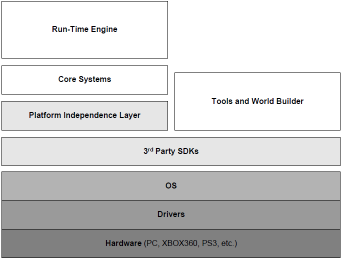
\includegraphics[width=0.5 \linewidth]{PICs/tools_arch_standalone.png}
		\caption{Standlone tool-suite}
		\label{fig:tools_standalone}
	\end{subfigure}%
	\begin{subfigure}{0.5\textwidth}
		\centering
		\centering 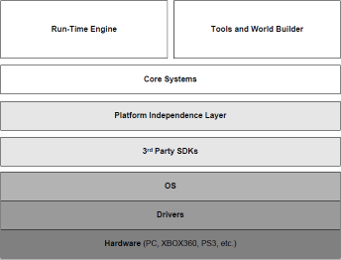
\includegraphics[width=0.5 \linewidth]{PICs/tools_arch_integrated.png}
		\caption{Integrated tool-suite on top of core systems}
		\label{fig:tools_integrated}
	\end{subfigure}
	
	\caption{Illustrated tool-suite architecture approaches commonly found among most engines}
\end{figure}

\noindent 
Beside these two kinds of architecture there is a third one that is almost uniquely used by \ac{UE4} and its previous versions. The developers at Epic went one step further and integrated the \textit{UnrealEd} directly into the engine's runtime. Having the benefit of total access to the systems and data structures, it simplifies the situation if having multiple representations of the same objects even more. Furthermore it is faster than other solutions when the game is run from withing the editor. That is due to the fact the part of the game is already running when the editor is integrated deeply into the engine's runtime. But with the power that approach established comes a great drawback. Because the tools are tightly coupled with the runtime, as soon as the game crashes or runs into an undefined state it also impacts the stability of the tools and sometimes even crashes them too, leading to a decrease of productivity and iteration times.


\subsection{Asset conditioning pipeline}

Being one of the tools that is included in almost every engine, the asset conditioning pipeline is responsible for formating the assets into a format that is better suited for the engine or a specific platform. Assets are normally generated using \ac{DCC} tools, including well-known solutions like Maya (3D modeling), Photoshop (Textures) or Audacity (Sound and Audio). The data that is created withing the \ac{DCC} tool is then exported into a intermediate format which often needs further processing before it can be sent to the game engine. The additional work is needed because the formats are often verbose and the asset pipeline can apply optimizations that are helping the performance of the runtime engine. Some of these techniques convert intermediate formats into binary ones, allowing them to be parsed faster at runtime, or group together assets with similar properties to reduce the size of files that have to be read. If the engine works on multiple platforms it is also often the job of the asset pipeline to convert the files to formats better suiting the target platform of the current build. 
